\documentclass[10pt,a4paper]{article}
\usepackage{ibaconnect}
\docinfo{Software Requirement Specification}{1.1}{18 Nov 2026}

% \fr{id}{title}{description}{inputs}{outputs}{rationale}{priority}{dependencies}
\newcommand{\fr}[8]{%
  \par\smallskip\noindent\begin{tabularx}{\linewidth}{@{}>{\bfseries}p{22mm} >{\raggedright\arraybackslash}X@{}}
  \multicolumn{2}{@{}l}{\color{accent}\bfseries #1: #2}\\\midrule
  Description & #3\\ Inputs & #4\\ Outputs & #5\\ Rationale & #6\\ Priority & #7\\ Dependencies & #8\\\bottomrule
  \end{tabularx}\par\smallskip}
\newcommand{\vone}[1]{\textcolor{accent}{\small[v1.1: #1]}}

\begin{document}

\begin{center}
{\large Institute of Business Administration, Karachi}\\
Software Engineering, Fall 2026\\[14mm]
{\color{accent}\Huge\bfseries SOFTWARE REQUIREMENT SPECIFICATION}\\[6mm]
{\LARGE\bfseries IBA Connect}\\[2mm]
{\large A verified campus network for finding the right people at IBA}\\[10mm]
\begin{tabular}{ll}
\textbf{Team name:} NameNotFound & \textbf{Instructor:} Mr.\ Ahsan Jawed\\
\textbf{Class section:} 102110 & \textbf{Milestone:} Software Requirement Specification\\
\textbf{Version:} 1.1 & \textbf{Date:} 18 Nov 2026\\
\end{tabular}\\[10mm]
\textbf{Team members}\\[2mm]
\begin{tabular}{rll}
\toprule
\# & ERP ID & Name\\\midrule
1 & 30485 & Ahsan Haris\\
2 & 30609 & Ahmed Abdul Rahim\\
3 & 30546 & Ayaan Arif Nadeem\\
4 & 31565 & Muhammad Mujtaba Khurram\\
5 & 31669 & Shaharyar Ahmed\\
6 & 30523 & Ebad ur Rahman\\
\bottomrule
\end{tabular}
\end{center}

\section*{Revision history}
\begin{revisions}
1.0 & Oct 2026 & Team NameNotFound & Submitted SRS (PDF).\\
1.1 & 18 Nov 2026 & Ahmed Abdul Rahim & Rebuilt in LaTeX from v1.0 without changing the requirements, except: email provider Resend $\rightarrow$ Brevo; F7 Practice quizzes removed from scope (sprint planning, replacement to follow for Sprint 2); request limit and cooldown values (FR3.1), chat polling (FR3.8) and idle session limit (FR1.6) made specific; data model notes from the Sprint 1 implementation (6.1). Changes are marked \vone{\ldots}.\\
\end{revisions}

\newpage
\tableofcontents
\newpage

\section{Introduction}
This SRS is accompanied by the companion document \emph{System Diagrams and User Stories}, which holds all system diagrams, the use cases and the 40 user stories with acceptance criteria.

\subsection{Purpose}
This document defines the functional, non-functional, interface, data and domain requirements for developing IBA Connect, a verified, IBA-only web platform that helps current students and alumni find the specific person they need on campus: a study partner, a project teammate, a senior who has already taken a course, or an alumnus working in a field of interest. The platform also provides private study and project groups with shared resources and practice quizzes. It replaces scattered, batch-bound WhatsApp groups with a searchable, persistent campus network.

\subsection{Scope}
IBA Connect will:
\begin{itemize}
\item Verify identity through IBA university accounts so that only real IBA students and alumni are admitted.
\item Provide structured, self-declared profiles (batch, programme, department, courses, skills, bio).
\item Let users search a directory by name, skill, course, and availability to advise.
\item Support connection requests (send, accept, decline) followed by private one-to-one chat.
\item Provide a Need Board where users post time-bound needs and others respond.
\item Provide private, invite-only study/project groups with resource upload and download.
\item Let group members create manual practice quizzes (multiple choice and true/false), attempt them, and track personal score history. \vone{removed from scope; see Section 3.7}
\item Allow users to flag content and give administrators a simple panel to review reports.
\item Run as a responsive web application usable on desktop and phone browsers.
\end{itemize}
\textbf{Target audience:} current IBA students, senior peer mentors, IBA alumni, and administrators/moderators (the project team and course administrator).

\textbf{Out of scope for this version:}
\begin{itemize}
\item Native mobile applications (iOS or Android).
\item AI-generated quizzes from uploaded material (a future goal, not part of the SRS baseline).
\item Faculty, staff, and exchange students as users.
\item Algorithmic matching, scoring, ranking, or ``people you may know'' recommendations.
\item Public or unauthenticated access, payments, subscriptions, or monetisation.
\item Automated content moderation, group leaderboards or comparative score views, and short-answer quiz questions.
\item Verification of declared courses, skills, or grades (all profile data is self-declared).
\end{itemize}

\subsection{Definitions, Acronyms, and Abbreviations}
\begin{itemize}
\item \textbf{API:} Application Programming Interface
\item \textbf{SRS:} Software Requirement Specification
\item \textbf{MVP:} Minimum Viable Product
\item \textbf{REST:} Representational State Transfer
\item \textbf{OAuth:} Open Authorization, the delegated sign-in standard used with Microsoft
\item \textbf{Entra ID:} Microsoft Entra ID (formerly Azure Active Directory), the identity provider used for sign-in
\item \textbf{RLS:} Row-Level Security (PostgreSQL access policies)
\item \textbf{ERD:} Entity Relationship Diagram
\item \textbf{IBA:} Institute of Business Administration, Karachi
\item \textbf{Verified user:} A user who has passed IBA identity verification (university sign-in, fallback email verification, or alumni verification)
\item \textbf{Senior / Peer Mentor:} A student who has enabled ``available to advise'' for specific courses
\item \textbf{Alumnus:} A graduate of IBA verified through the alumni process
\item \textbf{Need Board:} The shared board where verified users post time-bound needs
\item \textbf{Soft delete:} Removal from user view while the record is retained for recovery or audit
\item \textbf{p95:} 95th percentile response time
\item \textbf{FR / NFR / DR / UC / US:} functional requirement, non-functional requirement, domain requirement, use case, user story
\end{itemize}

\subsection{Intended Audience and Reading Guide}
\begin{itemize}
\item \textbf{Developers (team NameNotFound):} Sections 3, 5 and 6 define what to build and how data is stored.
\item \textbf{Product owner and instructor:} Sections 1, 2 and 3 and the appendices confirm the agreed scope.
\item \textbf{Testers:} Section 3 and the user stories (acceptance criteria) in the companion document, and Section 4 (measurable targets).
\item \textbf{Moderators and administrators:} FR8 and the administrator user class in Section 2.3.
\end{itemize}

\section{Overall Description (System Overview)}
\subsection{Product Perspective}
IBA Connect is a new, standalone web application. It is not integrated with IBA's student information system and has no access to official student, course or alumni data. It replaces informal, batch-bound WhatsApp groups with a searchable, persistent, verified network. It depends on external services: Microsoft Entra ID (sign-in), Supabase (database, auth, storage), Brevo (email) \vone{was Resend} and Vercel (hosting). The context diagram shows the people and services that exchange data with the system.

\begin{figure}[h]
\centering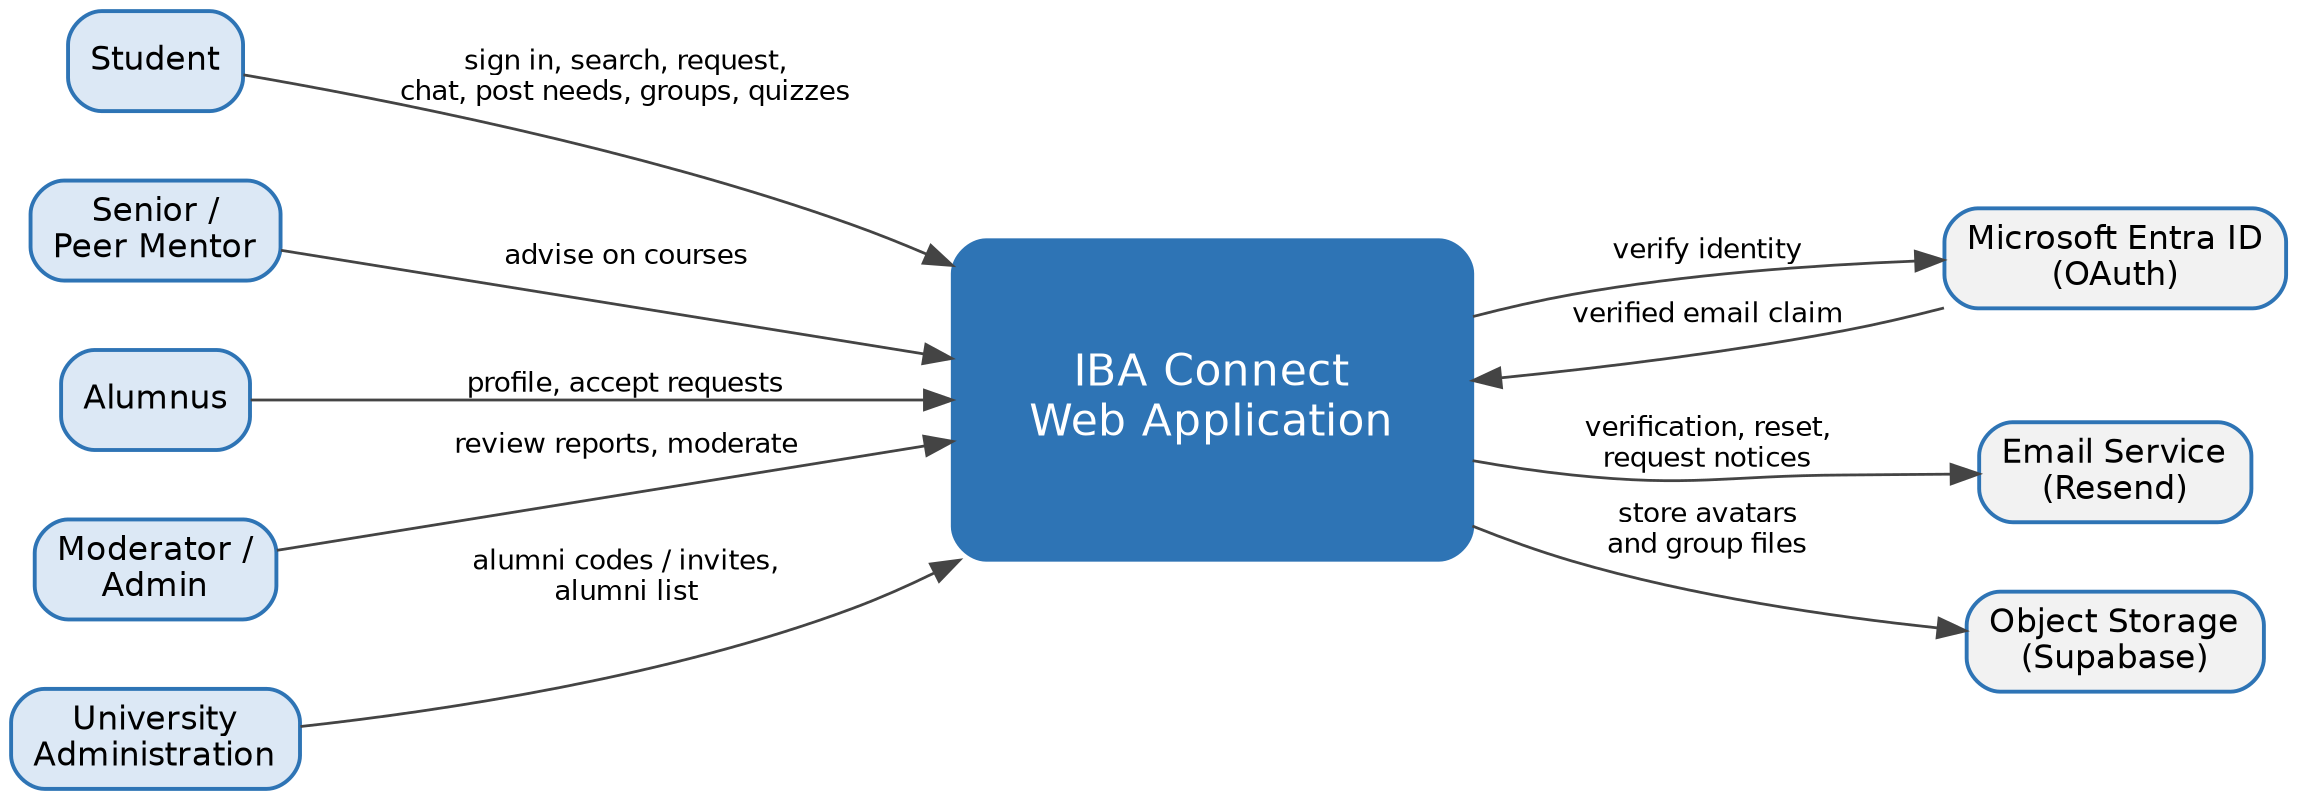
\includegraphics[width=\linewidth]{figures/context.png}
\caption{Context diagram of IBA Connect. (The email service shown as Resend is Brevo from v1.1.)}
\end{figure}

\subsection{Product Functions}
\begin{enumerate}
\item Verified sign-in for students and alumni, with an email-and-password fallback.
\item Self-declared profiles with courses, skills and an available-to-advise flag.
\item Directory browsing, free-text search and combinable filters.
\item Connection requests followed by private one-to-one chat.
\item A Need Board for time-bound requests (14-day expiry).
\item Private, invite-only groups with file sharing.
\item Manual practice quizzes with personal score history. \vone{removed from scope}
\item Content reporting and an admin moderation panel.
\end{enumerate}
Delivery follows a fixed build order: profiles and search, then connection requests and chat, then the Need Board, then groups and resources, then quizzes.

\subsection{User Classes and Characteristics}
All users hold the same kind of profile regardless of sign-in method.

{\small
\begin{tabularx}{\linewidth}{@{}>{\raggedright\arraybackslash}p{22mm} >{\raggedright\arraybackslash}X >{\raggedright\arraybackslash}X >{\raggedright\arraybackslash}p{18mm}@{}}
\toprule
\textbf{User class} & \textbf{Description} & \textbf{Key capabilities} & \textbf{Technical expertise}\\\midrule
Student & Current IBA student; signs in with an IBA Microsoft account or the fallback email & Profile, search, requests, chat, need board, groups, quizzes, reporting & Low to medium\\
Senior / Peer Mentor & Student with ``available to advise'' enabled for chosen courses & Everything a student can do, plus an advisor badge in search & Low to medium\\
Alumnus & Verified through an admin-issued code or invite, or a personal email matched against the alumni list & Same as a student; profile also holds field and company & Low to medium\\
Moderator / Administrator & The project team and the course administrator & Review reports, hide or remove content, warn, suspend, issue alumni codes & Medium to high\\
\bottomrule
\end{tabularx}}

\subsection{System Architecture}
IBA Connect is a responsive web application with its own versioned REST API (\texttt{/api/v1}). It is built with Next.js, React and TypeScript, uses PostgreSQL (hosted on Supabase) through the Prisma ORM, and is deployed to Vercel. Sign-in uses Microsoft Entra ID OAuth through Supabase Auth, with the IBA email domain (\texttt{khi.iba.edu.pk}) enforced server-side on the verified email claim. Transactional email is sent through Brevo \vone{was Resend}, and uploaded files and profile images are held in Supabase object storage.

\begin{figure}[h]
\centering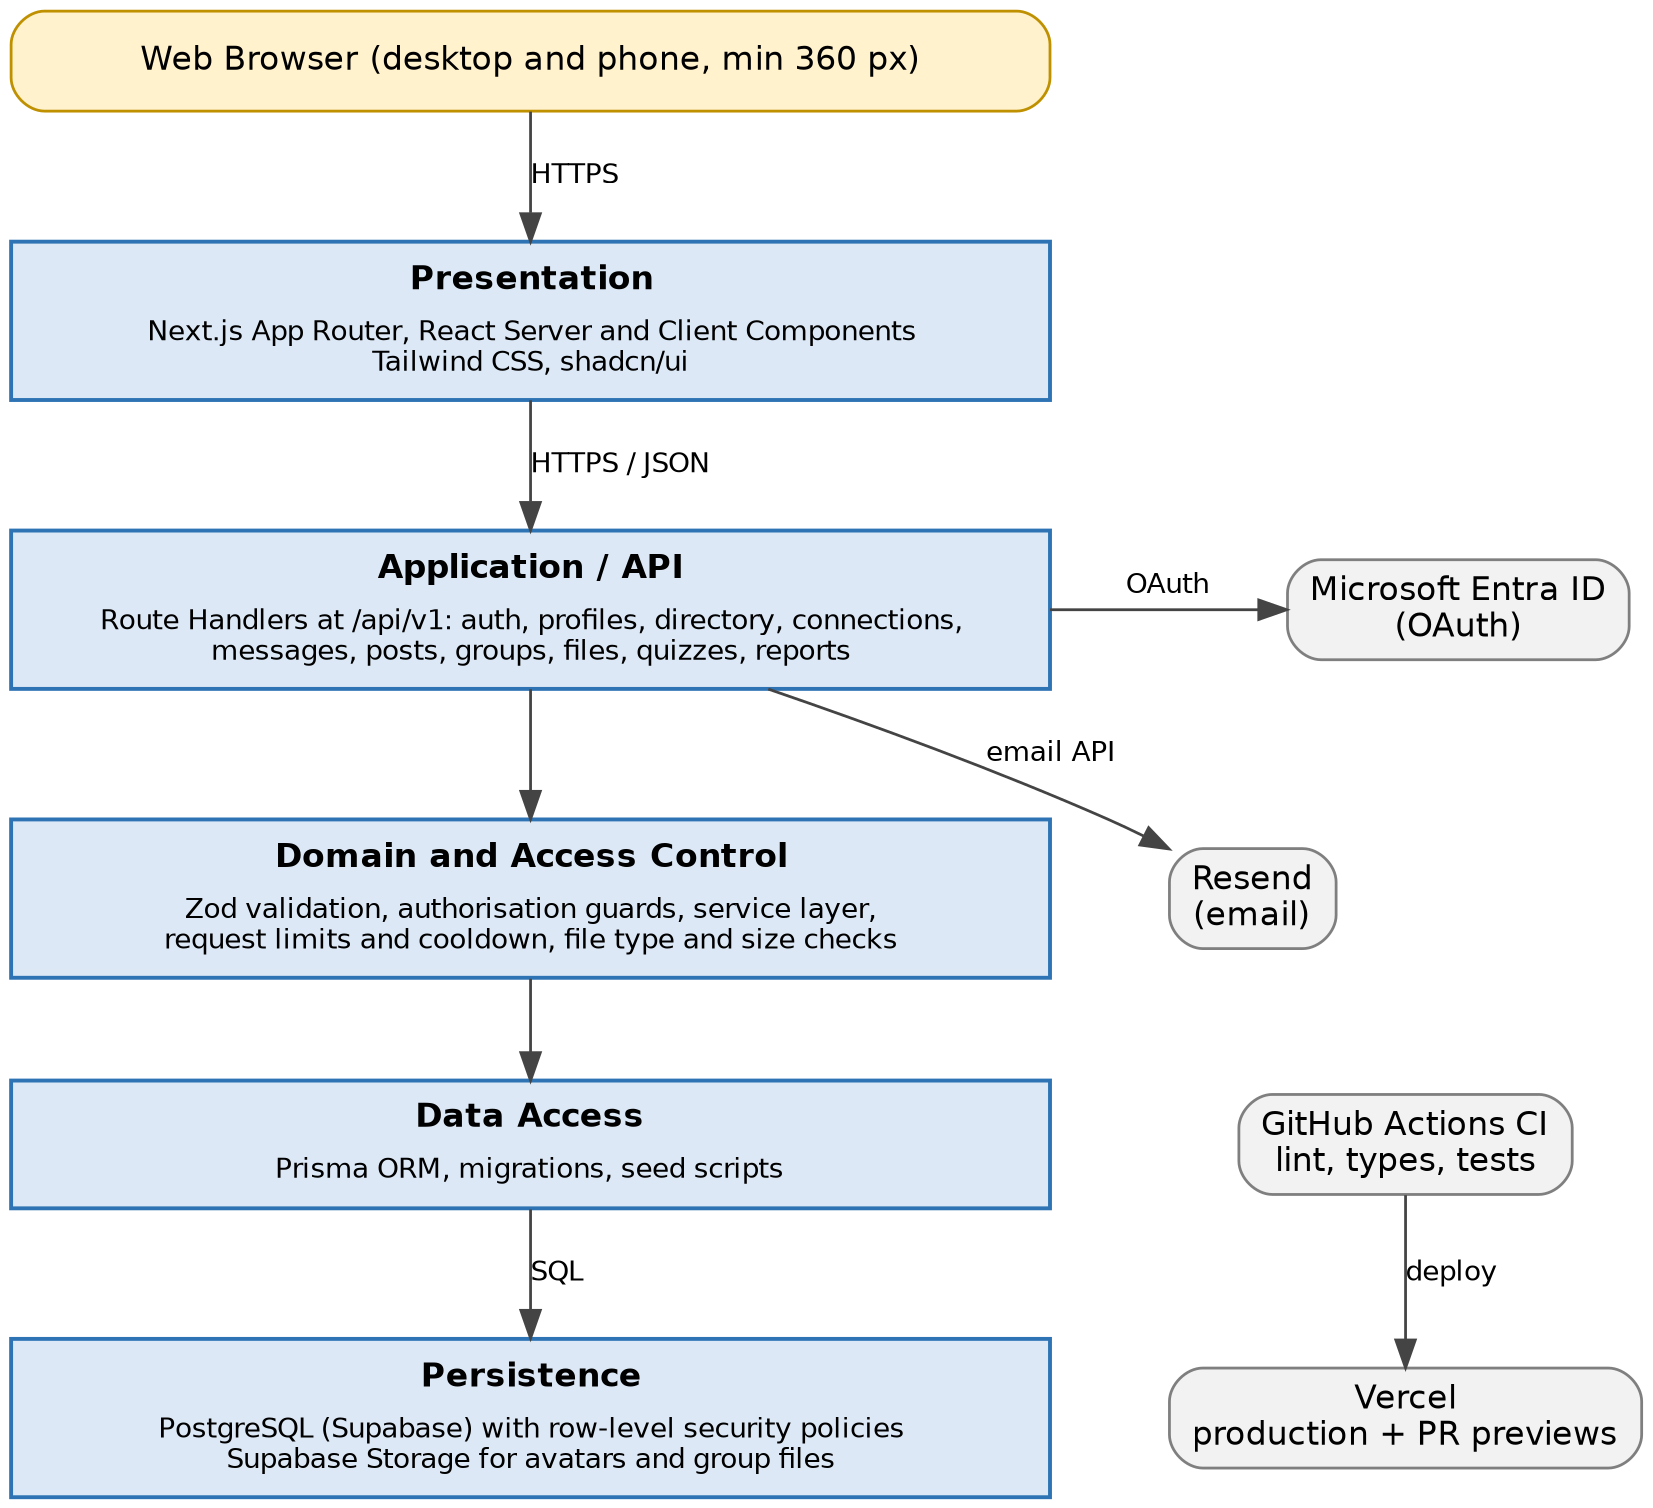
\includegraphics[width=0.75\linewidth]{figures/architecture.png}
\caption{Layered architecture and deployment topology. (Email: Brevo from v1.1.)}
\end{figure}

\subsection{Operating Environment}
\begin{itemize}
\item \textbf{Client:} current versions of Chrome, Edge, Firefox and Safari on desktop, Android and iOS (responsive web, minimum 360\,px width).
\item \textbf{Server:} Vercel (Next.js), Supabase (PostgreSQL, Auth, Storage) and Brevo (email) \vone{was Resend}, all on free tiers.
\end{itemize}

\subsection{User Documentation}
A short in-app help page and a README covering setup, environment variables and the seeded demo data. The REST API is documented in an OpenAPI specification.

\section{Functional Requirements}
This section defines the functional capabilities that IBA Connect shall provide. Each requirement is described with inputs, outputs, rationale, priority, and dependencies where applicable. User stories with acceptance criteria for each requirement are in the companion document (traceability in Appendix A1).

\subsection{Identity and Verified Profile}
\fr{FR1.1}{University Sign-In}{The system shall allow users to sign up and sign in with their university email or Microsoft sign-in (Microsoft Entra ID OAuth). The IBA email domain shall be enforced server-side on the returned verified email claim, and all other accounts shall be rejected.}{Microsoft account credentials (entered at Microsoft, never handled by the system).}{Authenticated session and a user profile record.}{The trust model rests on membership being limited to real IBA accounts.}{High}{Microsoft Entra ID, Supabase Auth.}
\fr{FR1.2}{Email and Password Fallback}{The system shall provide an email-plus-password fallback with email verification, forgot-password, and change-password flows for people who cannot use the university account. It shall produce the same kind of profile as Microsoft sign-in.}{Email, password, verification link, reset request.}{Verified account, confirmation or reset emails.}{Ensures access for people who cannot use the university account and serves as the fallback if Entra ID integration fails.}{High}{Transactional email service (Brevo \vone{was Resend}).}
\fr{FR1.3}{Alumni Verification}{The system shall verify alumni without requiring an active IBA email, either through a code or invite issued by the administration or by matching a personal email against an alumni list supplied by the university.}{Alumni code or invite, or personal email address.}{Verified alumnus account.}{Alumni typically no longer hold active IBA email accounts.}{High}{Administration-issued codes or invites; university-supplied alumni list.}
\fr{FR1.4}{Profile Creation and Editing}{The system shall let users create and edit a profile. Required fields: name, batch, programme and department, current semester, short bio, and skills. Optional but encouraged: courses taken, avatar, and the available-to-advise flag with courses. Alumni profiles shall also hold field and company. All data is self-declared and not verified.}{Profile field values and an optional avatar image.}{Saved profile and a profile view for other verified users.}{Structured profiles are what make search by course and skill possible.}{High}{Course list (seeded), object storage for avatars.}
\fr{FR1.5}{Available to Advise}{The system shall provide an available-to-advise toggle that also lets users select the specific courses they can help with. It shall be shown as a badge on profiles and as a search filter, not as a separate list.}{Toggle state and selected courses.}{Badge on profile and results; filterable attribute.}{Course-level availability is what makes advisor search useful.}{High}{FR1.4.}
\fr{FR1.6}{Sign Out and Session Handling}{The system shall let users sign out, shall expire idle sessions, and shall end the sessions of suspended users. \vone{the idle limit is configurable; 7 days is proposed, to be confirmed by the team}}{Sign-out action; session activity.}{Ended session; redirect to the sign-in page.}{Basic account security; needed for FR8.3.}{High}{Supabase Auth.}
\fr{FR1.7}{Dashboard}{The system shall provide a dashboard after sign-in showing pending requests, unread messages, the user's open need posts, and shortcuts to the directory, board and groups.}{Signed-in session.}{Dashboard page.}{NFR14 (three clicks from the dashboard) assumes a dashboard, but no requirement defined one.}{High}{FR3.3, FR3.4, FR4.1.}
\fr{FR1.8}{Account Deactivation and Deletion}{The system shall let a user deactivate or delete their account. The profile shall leave the directory immediately; records kept for audit (reports, admin actions) shall be anonymised.}{Deactivate or delete action with confirmation.}{Removed profile; anonymised retained records.}{Gives members control over their data.}{Medium}{FR1.4, Section 6.5.}
\fr{FR1.9}{Alumni Code Management}{Administrators shall be able to create, list, expire and revoke alumni codes and invites, and to upload the university-supplied alumni list.}{Code settings; alumni list file.}{Active, expired or revoked codes; stored alumni records.}{FR1.3 depends on codes and a list, but nothing defined who manages them.}{High}{FR1.3.}
\fr{FR1.10}{Course List Management}{Administrators shall be able to add, edit and retire courses in the seeded course list.}{Course code, title and department.}{Updated course list.}{The course list is team-maintained, with no official IBA data feed.}{Medium}{FR1.4.}

\subsection{Directory and Search}
\fr{FR2.1}{Browse Directory and View Profiles}{The system shall provide a paginated directory of verified members, with each result linking to a profile view visible only to signed-in verified users. Contact details shall never be shown in the directory.}{Page and sort selection.}{Paginated member cards and profile pages.}{Discovery of people is the core purpose of the platform.}{High}{FR1.4.}
\fr{FR2.2}{Free-Text Search}{The system shall support free-text search across name, skill, and course.}{Search keywords.}{Matching members.}{Lets users find someone quickly without knowing which filter to use.}{High}{FR2.1.}
\fr{FR2.3}{Search Filters}{The system shall provide combinable filters, in order of priority: course, skill, availability to advise, batch, and department/programme. For alumni, field and company filters shall be added.}{One or more filter values.}{Filtered, paginated results.}{Course comes first because finding a senior who has taken a course is the main use case.}{High}{FR1.4, FR1.5.}

\subsection{Connections and Messaging}
A connection request moves through the states below. The daily limit and cooldown in FR3.1 apply when a request is sent and after one is declined.
\begin{figure}[h]
\centering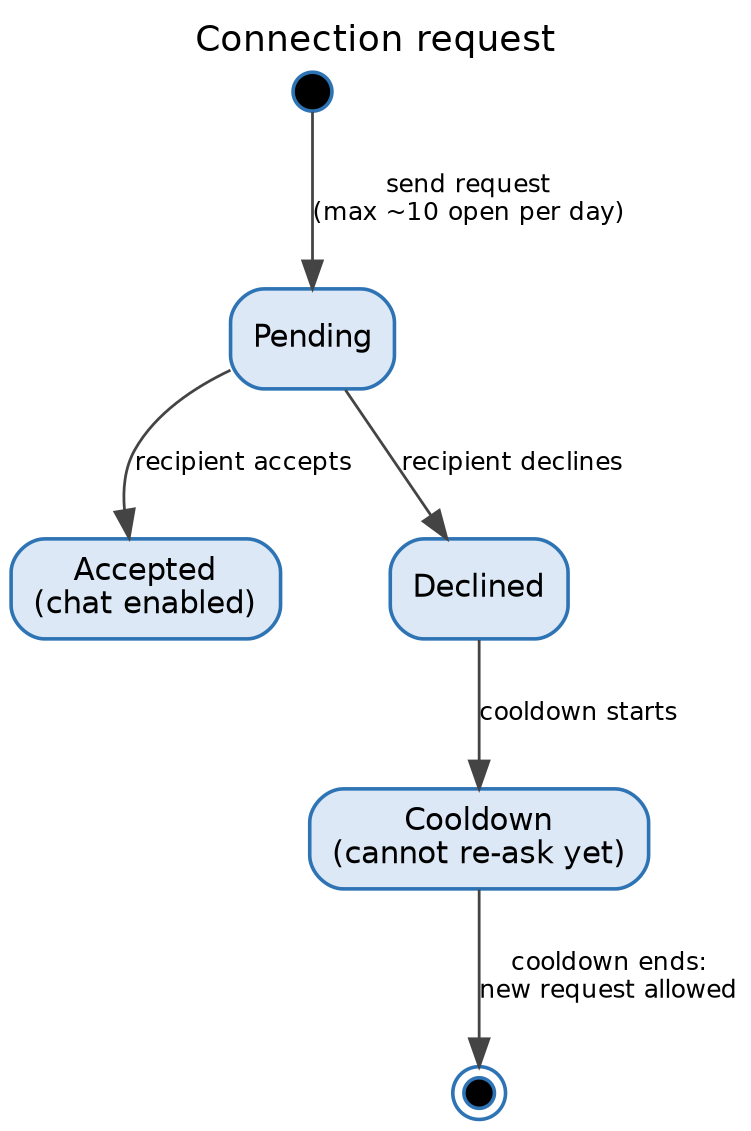
\includegraphics[width=0.45\linewidth]{figures/connection-states.png}
\caption{States of a connection request.}
\end{figure}

\fr{FR3.1}{Send Connection Request}{The system shall let a verified user send a connection request with a short context note. The system shall limit users to about ten open requests per day and apply a short cooldown before the same person can be asked again. \vone{at most 10 requests in any 24 hours; 3 days after a decline before asking the same person again (wireframe P07)}}{Recipient, context note.}{Pending request; email notification to the recipient.}{Limits spam and repeated asking.}{High}{FR1.4, FR2.1, transactional email.}
\fr{FR3.2}{Accept or Decline Request}{The recipient shall be able to accept or decline a request. Only after acceptance shall private chat be enabled between the two users.}{Accept or decline action.}{Updated request status; chat enabled on acceptance.}{Gives people control over who can message them.}{High}{FR3.1.}
\fr{FR3.3}{Requests Inbox}{The system shall provide a requests inbox with incoming, outgoing, and accepted views.}{View selection.}{Lists of requests by status.}{Lets members keep track of who they have asked and who has asked them.}{High}{FR3.1.}
\fr{FR3.4}{Private One-to-One Chat}{The system shall provide a private message thread between accepted connections only, with unread indicators.}{Message text.}{Stored messages in the thread; unread counts.}{Moves conversations off scattered WhatsApp groups while keeping them private.}{High}{FR3.2.}
\fr{FR3.5}{Contact Visibility}{A member's email address shall become visible to another member only after a connection is accepted.}{Accepted connection.}{Email shown on the connected member's profile.}{Protects member privacy.}{High}{FR3.2.}
\fr{FR3.6}{Notifications}{The system shall send an email notification for a new connection request and shall show in-app unread indicators for requests and messages.}{New request or message event.}{Email; unread badges.}{Members need to know when someone is waiting for a reply.}{Medium}{FR3.1, FR3.4, Brevo \vone{was Resend}.}
\fr{FR3.7}{Block User}{A user shall be able to block another user, which prevents new requests and messages from them.}{Block action.}{Block record; refused requests and messages from the blocked user.}{Gives members a direct way to stop unwanted contact before a moderator acts.}{Medium}{FR3.1, FR3.4.}
\fr{FR3.8}{Chat Constraints}{Chat shall be text only, with a maximum message length of 2,000 characters. New messages shall appear by polling or a real-time subscription; the choice is a design decision for Sprint 2. \vone{decided: polling every 5 seconds}}{Message text.}{Accepted or rejected message.}{Keeps chat simple and within free-tier limits.}{Medium}{FR3.4.}

\subsection{Need Board}
\fr{FR4.1}{Create Need Post}{The system shall let a verified user create a time-bound post of a defined type (study partner, project teammate, course advice, career advice), with an optional course or department tag. Posts shall be visible to all verified users.}{Type, title, body, optional course/department tag.}{Open post on the board.}{Lets people ask for help without knowing who to message.}{High}{FR1.4.}
\fr{FR4.2}{Browse and Filter Board}{The system shall let users browse the open posts and filter them by type and by course or department tag.}{Filter criteria.}{List of open posts.}{Helps people find needs they can answer.}{High}{FR4.1.}
\fr{FR4.3}{Respond to a Post}{The system shall let a user respond to a post, which opens a connection request pre-filled with the post context. The same request limits as FR3.1 apply.}{Response message.}{Connection request linked to the post.}{Reuses the connection flow so the privacy rules stay the same.}{High}{FR3.1.}
\fr{FR4.4}{Close and Expire Posts}{Posts shall auto-expire after 14 days, and the poster may close a post early. Responses shall remain visible to the poster after closing, but the post shall leave the open list.}{Close action; elapsed time.}{Closed or expired post; retained responses.}{Keeps the board current.}{High}{FR4.1.}
\fr{FR4.5}{Edit Own Post}{A poster shall be able to edit the title, body and tag of their open post.}{Updated post fields.}{Updated post.}{Lets posters fix mistakes without closing and reposting.}{Low}{FR4.1.}

\subsection{Study and Project Groups}
\fr{FR5.1}{Create Group}{Any verified user may create a group. Study groups and project groups are the same feature, with a type label that changes no behaviour. No prior connection or shared course is required.}{Group name, type label, description.}{New group with the creator as group admin.}{Lets people organise work without any gatekeeping.}{High}{FR1.4.}
\fr{FR5.2}{Private, Invite-Only Membership}{Groups shall be fully private and invite-only. They shall not appear in search. Members shall be added by invite link or by the creator.}{Invite link or creator action.}{Updated membership.}{Keeps group work private to the people invited.}{High}{FR5.1.}
\fr{FR5.3}{Member-Only Content}{Group content (files and quizzes) shall be visible only to group members.}{Request for group content.}{Content for members; refusal for everyone else.}{Keeps study material within the group.}{High}{FR5.2.}
\fr{FR5.4}{Member Management}{The group admin shall be able to remove members and to revoke or regenerate the invite link. Members shall be able to leave a group.}{Remove, revoke, regenerate or leave action.}{Updated membership; invalidated old link.}{An invite-only group needs a way to end access once a link is shared or a member should go.}{High}{FR5.2.}
\fr{FR5.5}{Group Deletion and Admin Transfer}{The creator shall be able to delete the group (soft delete) or transfer the admin role to another member.}{Delete or transfer action.}{Hidden group, or a new group admin.}{Prevents orphaned groups when the creator leaves.}{Medium}{FR5.1.}

\subsection{Resource Sharing}
\fr{FR6.1}{Upload Resources}{Any group member may upload files of type PDF, DOCX, PPTX, and images, up to 25 MB per file. Archives and executables shall be rejected.}{File.}{Stored file listed in the group.}{Shared notes and slides are the main reason groups exist.}{High}{Object storage, FR5.3.}
\fr{FR6.2}{Download Resources}{Group members shall be able to view and download files in their group through signed, time-limited links.}{Download request.}{File download.}{Signed links stop files being shared outside the group.}{High}{FR6.1.}
\fr{FR6.3}{Delete Resources}{Only the uploader or the group admin (the creator) may delete a file. Deletion shall be a soft delete so the file can be recovered or audited.}{Delete action.}{File hidden from members; record retained.}{Allows removal of mistakes while keeping an audit trail.}{Medium}{FR6.1.}

\subsection{Practice Quizzes}
\vone{F7 Practice quizzes was removed from scope at sprint planning. A replacement feature will be specified for Sprint 2. The original requirements are kept below for traceability.}
\fr{FR7.1}{Create Quiz}{Group members shall create quiz questions manually. Supported question types are multiple choice and true/false.}{Quiz title, questions, answer options, correct answers.}{Saved quiz in the group.}{Turns shared material into practice.}{High}{FR5.3.}
\fr{FR7.2}{Attempt Quiz}{Group members shall be able to attempt a quiz and receive a score.}{Selected answers.}{Score and result.}{Lets members test their understanding.}{High}{FR7.1.}
\fr{FR7.3}{Personal Score History}{The system shall show each user a list of their attempts per quiz with score and date, plus a simple chart of their scores over time. Scores are personal only, with no group leaderboards or comparisons.}{Quiz selection.}{Attempt list and score chart.}{Lets members track progress without competition.}{Medium}{FR7.2.}
\fr{FR7.4}{Manage Quizzes}{The quiz author or the group admin shall be able to edit or delete a quiz (soft delete). Attempt history shall be retained.}{Edit or delete action.}{Updated or hidden quiz.}{Authors need to correct mistakes in questions.}{Medium}{FR7.1.}
\fr{FR7.5}{Quiz Rules}{A quiz shall have at least one question. A multiple choice question shall have two to six options with exactly one correct answer. Members may retake a quiz any number of times, and each attempt is stored.}{Quiz content; attempts.}{Validated quiz; stored attempts.}{Fixes the quiz structure so scoring and score history are unambiguous.}{High}{FR7.1, FR7.2.}

\subsection{Moderation and Administration}
\fr{FR8.1}{Report Content}{Users shall be able to flag profiles, messages, need-board posts, group files, quizzes, and groups.}{Target item and reason.}{Report in the admin queue.}{Community reporting is the main safeguard, since there is no automated moderation.}{Medium}{None.}
\fr{FR8.2}{Admin Panel}{The system shall provide a simple admin panel, handled by the project team and the course administrator, where reports can be reviewed. Available actions: hide or remove content, warn, and suspend. There is no automated moderation.}{Report and chosen action.}{Updated content or account status.}{Gives moderators one place to act on reports.}{Medium}{FR8.1.}
\fr{FR8.3}{Effect of Moderation Actions}{A suspended user shall be unable to sign in, and their content shall be hidden but retained. A warned user shall see the warning at next sign-in.}{Warn or suspend action.}{Changed account status; warning message.}{FR8.2 names the actions but not what they do.}{Medium}{FR8.2, FR1.6.}
\fr{FR8.4}{Audit Log}{The system shall record every administrator action (who, what, when, on which item).}{Administrator action.}{Audit record.}{Makes moderation accountable and reviewable.}{Medium}{FR8.2.}
\fr{FR8.5}{Admin Role Assignment}{Administrator accounts shall be assigned through seeded configuration or a database-level change, not through self-service.}{Seed or configuration change.}{Account with the admin role.}{Prevents anyone from granting themselves moderator powers.}{High}{FR1.1.}

\section{Non-Functional Requirements}
\subsection{Performance}
\begin{itemize}
\item \textbf{NFR1:} Directory search shall return results within 2 seconds at the 95th percentile.
\item \textbf{NFR2:} The system shall be sized for current students and alumni together, with a design load of a few thousand users (not the entire university at once). Performance shall be tested on a seeded dataset of 1,000 members.
\end{itemize}
\subsection{Reliability}
\begin{itemize}
\item \textbf{NFR3:} Availability is best-effort on free hosting tiers; no uptime guarantee is claimed or tested.
\item \textbf{NFR4:} Deleted group files shall be soft-deleted so they can be recovered or audited.
\item \textbf{NFR19:} Database backups shall rely on the Supabase free-tier facilities; no recovery time objective is promised, consistent with NFR3.
\end{itemize}
\subsection{Security}
\begin{itemize}
\item \textbf{NFR5:} All communications shall use HTTPS.
\item \textbf{NFR6:} Passwords, where used, shall be hashed with bcrypt.
\item \textbf{NFR7:} Authorisation shall be enforced server-side on every API route and reinforced by PostgreSQL row-level security policies, with no reliance on client-side checks.
\item \textbf{NFR8:} The IBA email domain restriction shall be enforced server-side on the verified email claim.
\item \textbf{NFR9:} Uploaded files shall be validated against the allowed types and 25 MB limit, and accessed only through signed URLs.
\item \textbf{NFR18:} The server shall log authentication failures and administrator actions. Logs shall not contain passwords or message content.
\item \textbf{NFR20:} The API shall rate-limit sign-in, registration and password-reset endpoints to reduce abuse.
\end{itemize}
\subsection{Privacy}
\begin{itemize}
\item \textbf{NFR10:} Contact details shall never be exposed in the directory. A member's email shall be visible to another member only after a connection is accepted.
\item \textbf{NFR11:} No content shall be visible without a verified sign-in, and groups shall be visible only to their members.
\item \textbf{NFR22:} Retention and deletion of data shall follow Section 6.5.
\end{itemize}
\subsection{Scalability}
\begin{itemize}
\item \textbf{NFR12:} The system shall handle the design load in NFR2 on the free-tier infrastructure, with the seeded demonstration dataset sized to stay within free-tier limits.
\end{itemize}
\subsection{Usability}
\begin{itemize}
\item \textbf{NFR13:} All primary flows shall be usable at a 360\,px viewport width.
\item \textbf{NFR14:} Every screen shall be reachable within three clicks of the dashboard (see FR1.7).
\item \textbf{NFR16:} The application shall work on the two latest major versions of Chrome, Edge, Firefox and Safari.
\item \textbf{NFR17:} Primary flows shall meet WCAG 2.1 AA basics: keyboard navigation, visible focus, text alternatives for images, and sufficient colour contrast.
\end{itemize}
\subsection{Maintainability}
\begin{itemize}
\item \textbf{NFR15:} Lint and type-check shall be enforced in CI, with no direct commits to main; every change shall be merged through a reviewed pull request.
\item \textbf{NFR21:} Each High-priority functional requirement shall have at least one automated test or a documented manual test case.
\end{itemize}

\section{External Interface Requirements}
\subsection{User Interface (UI)}
\begin{itemize}
\item IBA Connect shall be a responsive web application accessible on desktop browsers and on mobile phone browsers (no native Android or iOS applications).
\end{itemize}
\subsection{Software Interfaces (APIs)}
\begin{itemize}
\item The system shall expose its own versioned REST API under \texttt{/api/v1} (auth, profiles, directory, connections, messages, posts, groups, files, quizzes, reports), documented in an OpenAPI specification.
\item The system shall connect with:
  \begin{itemize}
  \item Microsoft Entra ID OAuth (sign-in and identity verification).
  \item Brevo (verification, password reset, and connection-request emails) \vone{was Resend}.
  \item Supabase Storage (profile images and group files).
  \end{itemize}
\end{itemize}
\subsection{Hardware Interfaces}
\begin{itemize}
\item The system shall be deployed on cloud platforms (Vercel for the application, Supabase for database and storage). No special hardware is required.
\end{itemize}
\subsection{Communication Interfaces}
\begin{itemize}
\item Browser to server over HTTPS (TLS), using JSON over the REST API under \texttt{/api/v1}.
\item Microsoft Entra ID: OAuth 2.0 / OpenID Connect authorization code flow. The system receives and checks the verified email claim (\texttt{xms\_edov}) and never receives the Microsoft password.
\item Brevo \vone{was Resend}: HTTPS API calls from the server to send email; Supabase Auth emails through Brevo SMTP.
\item Supabase Storage: HTTPS signed URLs, valid for a short time (5 minutes).
\item Errors shall be returned in a consistent JSON shape with an HTTP status code and a message.
\end{itemize}

\section{Data Requirements}
The data model below matches the entity relationship diagrams in the companion document.

\subsection{Logical Data Entities}
{\small
\begin{longtable}{@{}p{24mm} >{\raggedright\arraybackslash}p{78mm} >{\raggedright\arraybackslash}p{48mm}@{}}
\toprule
\textbf{Entity} & \textbf{Key attributes} & \textbf{Notes}\\\midrule\endhead
User & id, iba\_email (unique), personal\_email, name, avatar\_url, role (student, alumnus, admin), batch, programme, department, semester, bio, available\_to\_advise, field, company, status (active, suspended), created\_at & Holds the profile; field and company are for alumni. FR1.8 adds a deactivated status\\
AlumniRecord & id, personal\_email, invite\_code, claimed\_by (FK to User) & Alumni list entries and admin-issued codes; one record is claimed by one user\\
Course & id, code, title, department & Seeded, team-maintained\\
UserCourse & user\_id, course\_id, semester\_taken, can\_advise & Courses taken, with the advise flag per course\\
Skill & id, name & Shared skill list\\
UserSkill & user\_id, skill\_id & Many-to-many link\\
Connection & id, requester\_id, recipient\_id, status (pending, accepted, declined), context\_note, origin\_post\_id (nullable), created\_at, responded\_at & Limit and cooldown checks use this table\\
Message & id, connection\_id, sender\_id, body, sent\_at, read\_at & Only for accepted connections\\
Post & id, author\_id, type (study partner, project teammate, course advice, career advice), course\_id (nullable), department\_tag, title, body, status (open, closed), expires\_at & expires\_at = created\_at + 14 days\\
PostResponse & id, post\_id, responder\_id, message, connection\_id, created\_at & Each response opens a Connection\\
Group & id, creator\_id, name, type\_label (study, project), description, invite\_token, created\_at & Creator is group admin. FR5.5 adds deleted\_at\\
GroupMember & group\_id, user\_id, role (admin, member), joined\_at & \\
Group file & id, group\_id, uploader\_id, file\_name, file\_type (pdf, docx, pptx, image), size\_bytes (max 25 MB), storage\_path, deleted\_at (soft delete), created\_at & Stored in Supabase Storage; the row holds the path\\
Quiz & id, group\_id, creator\_id, title, created\_at & FR7.4 adds deleted\_at\\
Question & id, quiz\_id, type (mcq, true\_false), text, position & True/false uses two fixed options\\
QuestionOption & id, question\_id, text, is\_correct & \\
QuizAttempt & id, quiz\_id, user\_id, score, total, attempted\_at & Personal only\\
AttemptAnswer & id, attempt\_id, question\_id, option\_id & \\
Report & id, reporter\_id, target\_type (profile, message, post, file, quiz, group), target\_id, reason, status (open, resolved), action (hide, remove, warn, suspend), handled\_by (FK to admin), created\_at & \\
Block & blocker\_id, blocked\_id, created\_at & Supports FR3.7\\
AdminAction & id, admin\_id, report\_id, action, created\_at & Audit trail for FR8.4\\
\bottomrule
\end{longtable}}

\vone{Sprint 1 implementation notes: \texttt{User.email} is the sign-in email (IBA, or personal for alumni) and \texttt{personalEmail} holds the alumni verification email; \texttt{avatarPath} stores a storage path, not a public URL; a \texttt{RateLimitHit} table holds rate-limit counters; \texttt{AdminAction} records target type and id so it also covers alumni code and course changes. Quiz entities are no longer needed (F7 removed). The current ERD is generated from the Prisma schema in the Architecture and Data Model document.}

\subsection{Key Relationships}
\begin{itemize}
\item A User has many courses (through UserCourse) and many skills (through UserSkill).
\item An AlumniRecord is claimed by at most one User.
\item A Connection links two Users; Messages belong to one accepted Connection.
\item A Post has many PostResponses; each response creates a Connection linked back to the Post.
\item A Group has many Members, files and Quizzes; a Quiz has many Questions, and a Question has many options.
\item A User has many QuizAttempts; each attempt has many AttemptAnswers.
\item A Report points to one target item (profile, message, post, file, quiz or group).
\end{itemize}
The first part of the ERD, covering users, profiles, courses, skills and alumni verification, is shown below. The other four parts (connections and messages, need board, groups and reports, quizzes) are in the companion document.
\begin{figure}[h]
\centering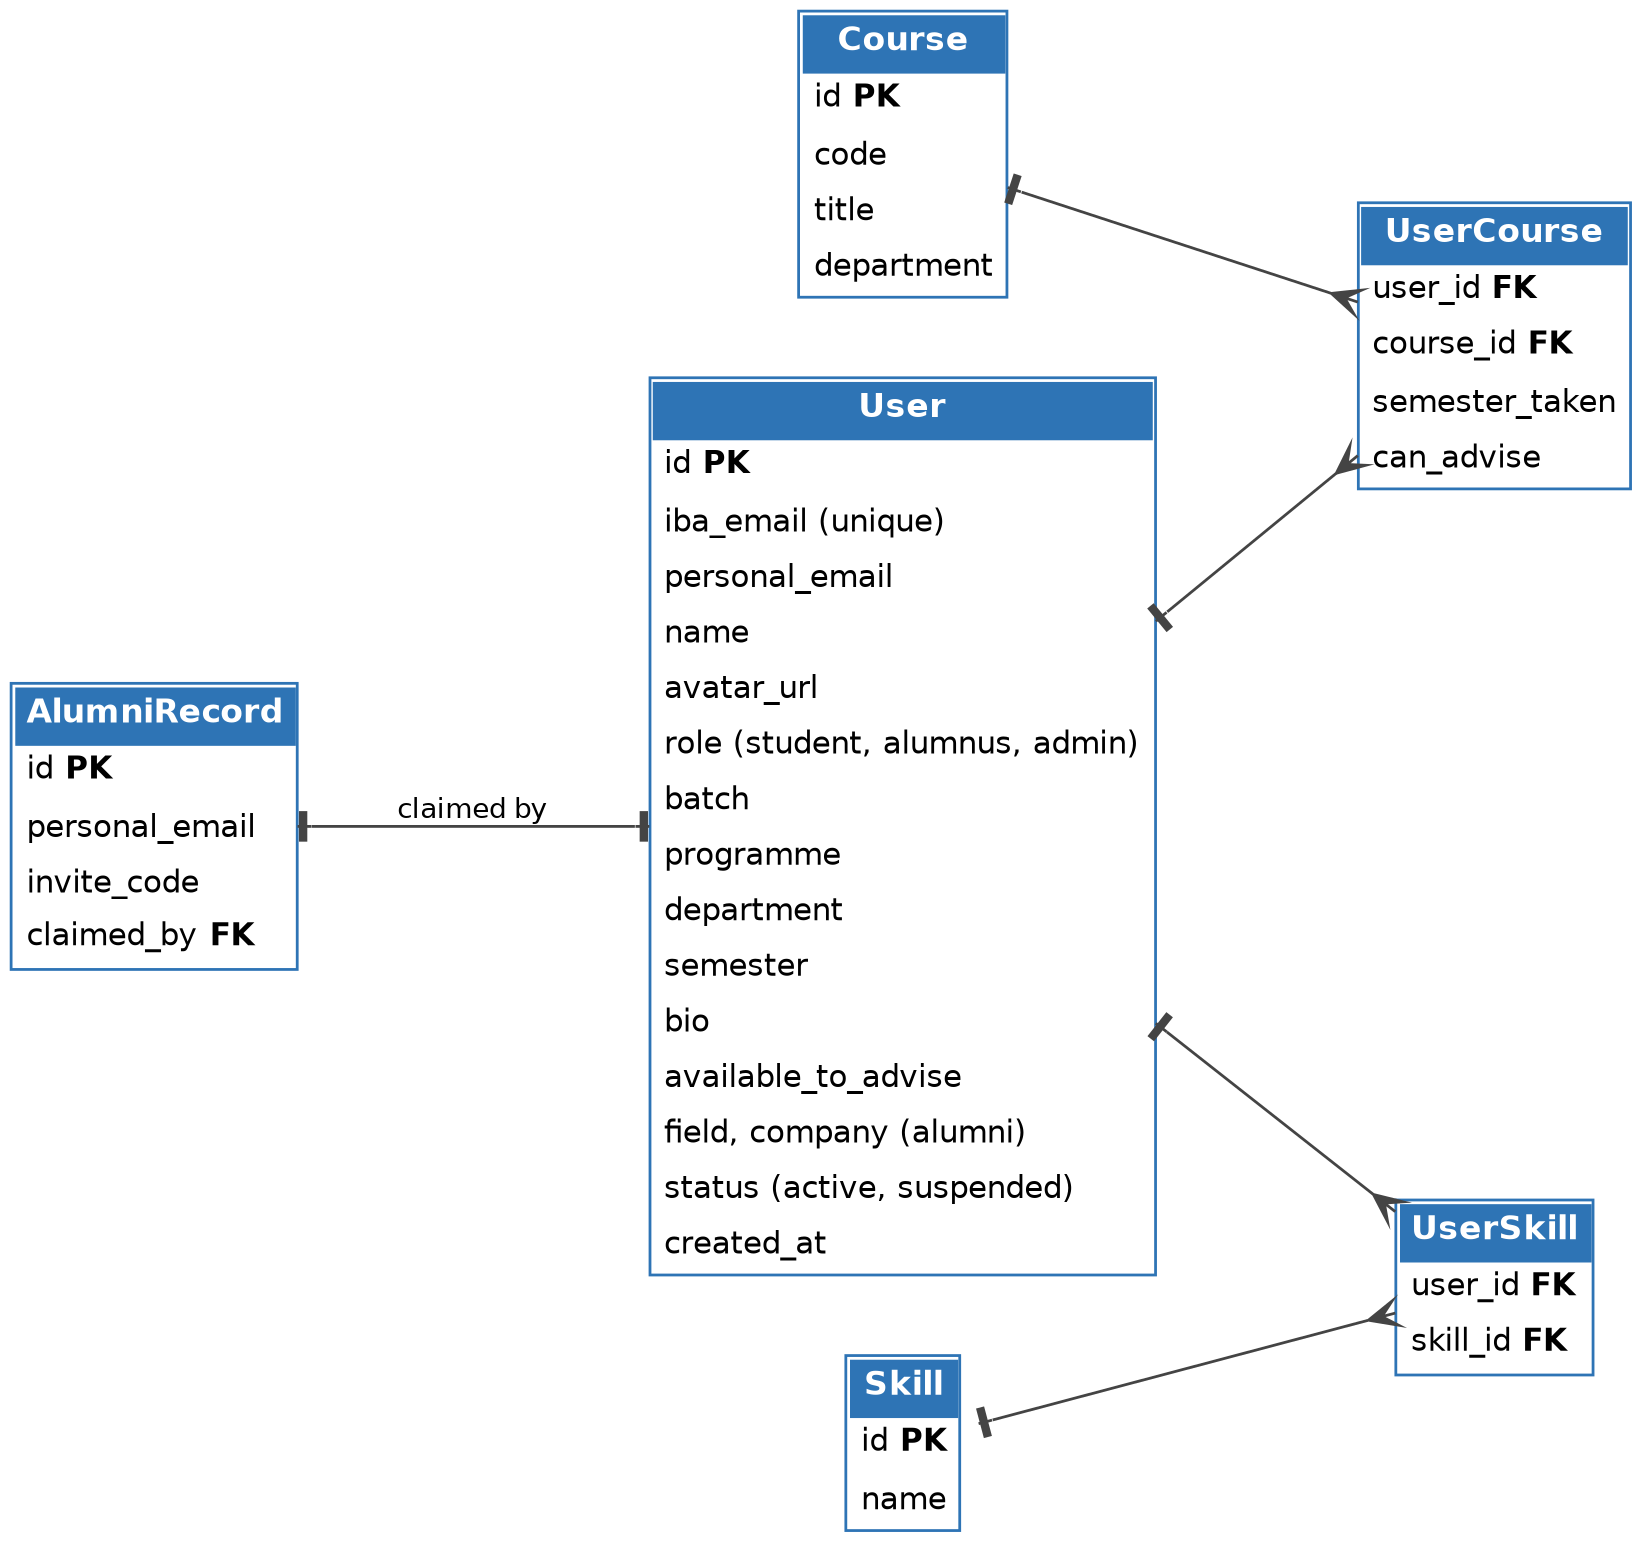
\includegraphics[width=0.8\linewidth]{figures/erd-part1.png}
\caption{ERD part 1: users, profiles, courses, skills and alumni verification.}
\end{figure}

\subsection{Data Validation Rules}
\begin{itemize}
\item \textbf{Email:} iba\_email must be unique; Microsoft sign-in requires the IBA domain and a verified email claim.
\item \textbf{Profile:} name, batch, programme, department, semester, bio and at least one skill are required (FR1.4). Bio maximum length: 500 characters.
\item \textbf{Connection request note:} maximum 300 characters; about ten open requests per user per day; a cooldown before the same person is asked again (FR3.1).
\item \textbf{Post:} type, title and body are required; expires\_at is 14 days after creation.
\item \textbf{File:} type must be PDF, DOCX, PPTX or an image, validated by extension and content type; maximum 25 MB.
\item \textbf{Quiz:} rules in FR7.5.
\end{itemize}
\subsection{Data Integrity and Access}
\begin{itemize}
\item Foreign keys and unique constraints are enforced in PostgreSQL through Prisma.
\item Row-level security policies restrict rows to authorised users (own profile edits, own messages, group members only for group content), reinforcing the server-side checks in NFR7.
\item Email addresses are returned by the API only for accepted connections (NFR10).
\end{itemize}
\subsection{Retention and Deletion}
\begin{itemize}
\item Soft-deleted files, quizzes and groups are kept for audit for 90 days and then purged.
\item Messages persist while both users remain active. When an account is deleted, its messages are anonymised.
\item Reports and admin actions are retained for the duration of the course project.
\item Expired or used alumni codes are retained for audit.
\end{itemize}
\subsection{Data Volume and Seed Data}
\begin{itemize}
\item Design load: a few thousand users; performance is tested on a seeded dataset of 1,000 members (NFR2).
\item Storage: group files of up to 25 MB each, within the Supabase free-tier storage limit.
\item Seed data: course list, department and programme list, and demonstration members. Seed data shall contain no real personal data.
\end{itemize}
\subsection{Data Privacy}
\begin{itemize}
\item All profile data is self-declared and shall not be shown as verified (DR2).
\item Passwords, where used, are stored only as bcrypt hashes (NFR6).
\item Uploaded files are accessible only through signed, time-limited URLs (NFR9).
\end{itemize}

\section{Domain Requirements}
\begin{itemize}
\item \textbf{DR1:} Only current IBA students and IBA alumni shall be admitted; faculty, staff, and exchange students are out of scope.
\item \textbf{DR2:} Profile data (courses, skills, grades, and roles) is self-declared and shall not be presented as verified.
\item \textbf{DR3:} Reported content shall be handled by the project team and the course administrator through the admin panel, using hide/remove, warn, or suspend actions.
\item \textbf{DR4:} Group file sharing shall be limited to PDF, DOCX, PPTX, and images, and shall not permit archives or executables.
\end{itemize}

\section{Constraints}
\begin{itemize}
\item Development shall follow the course timeline: Sprint 1 (2 Nov to 15 Nov 2026) and Sprint 2 (25 Nov to 6 Dec 2026), with mid-terms immediately preceding Sprint 1.
\item Features shall be built in this order: profiles and search, connection requests and chat, Need Board, groups and resources, then quizzes.
\item Only free tiers of Supabase, Vercel, and Brevo \vone{was Resend} may be used, which limit database size, monthly active users, and email volume.
\item Restricting sign-in to IBA's own Entra tenant requires an app registration students cannot create, so a multi-tenant app in the team's own tenant is used with server-side domain enforcement (confirming the \texttt{xms\_edov} claim). If this is not working by the end of Sprint 1, the fallback is email-domain validation plus an emailed verification link.
\item There is no access to official IBA student, course, or alumni data; reference data is team-maintained and self-declared.
\item The technology stack is Next.js, TypeScript, PostgreSQL (Supabase) with Prisma, Supabase Auth, and Vercel with GitHub Actions CI.
\end{itemize}

\section{Assumptions and Dependencies}
\begin{itemize}
\item Microsoft Entra ID will remain available and will return a verified email claim usable for domain checks.
\item The administration will issue alumni codes or invites, or the university will supply an alumni list for matching.
\item The course list will be seeded from a static, team-maintained list.
\item Users will provide honest, self-declared profile information.
\item The Brevo \vone{was Resend} email service will deliver verification and notification emails within free-tier limits.
\item Users will have stable internet connections.
\item Where this SRS differs from the earlier project proposal (groups, file sharing, quizzes, and moderation now in scope; alumni verification by code or alumni list; need board visible to all verified users), the product owner's answers take precedence.
\end{itemize}

\section{Appendices}
\subsection*{A1: Requirement Traceability}
{\small
\begin{tabularx}{\linewidth}{@{}>{\raggedright\arraybackslash}p{38mm} l l l >{\raggedright\arraybackslash}X@{}}
\toprule
\textbf{Requirement group} & \textbf{Build order} & \textbf{Client Q\&A} & \textbf{Use cases} & \textbf{User stories}\\\midrule
FR1 Identity and Profile & 1 & Q2, Q3, Q4, Q6 & UC1 to UC6 & US1.1 to US1.8\\
FR2 Directory and Search & 1 & Q5, Q18 & UC7, UC8 & US2.1 to US2.6\\
FR3 Connections and Messaging & 2 & Q7 & UC9 to UC11 & US3.1 to US3.7\\
FR4 Need Board & 3 & Q8 & UC12 to UC14 & US4.1 to US4.5\\
FR5 Groups & 4 & Q1, Q9, Q10 & UC15 to UC17 & US5.1 to US5.4\\
FR6 Resource Sharing & 4 & Q11, Q12 & UC18 to UC20 & US6.1 to US6.4\\
FR7 Quizzes \vone{removed} & 5 & Q13, Q14, Q15 & UC21 to UC23 & US7.1 to US7.3\\
FR8 Moderation and Admin & Medium priority & Q16 & UC24 to UC28 & US8.1 to US8.3\\
NFRs and Interfaces & All & Q17, Q18 & -- & --\\
\bottomrule
\end{tabularx}}

\subsection*{A2: Use Case Summary}
{\small
\begin{longtable}{@{}l >{\raggedright\arraybackslash}p{52mm} >{\raggedright\arraybackslash}p{38mm} l l@{}}
\toprule
\textbf{ID} & \textbf{Use case} & \textbf{Primary actor(s)} & \textbf{User stories} & \textbf{SRS requirement}\\\midrule\endhead
UC1 & Sign in with Microsoft & Student; Microsoft Entra ID & US1.1 & FR1.1\\
UC2 & Verify IBA domain (server-side) & System; Microsoft Entra ID & US1.1 & FR1.1\\
UC3 & Sign up with email and password, verify & Student, Alumnus & US1.2, US1.3 & FR1.2\\
UC4 & Verify alumni status & Alumnus; University Administration & US1.4 & FR1.3\\
UC5 & Create / edit profile & Verified User & US1.5, US1.6, US1.7 & FR1.4\\
UC6 & Set available to advise & Senior & US1.8 & FR1.5\\
UC7 & Search and filter directory & Verified User & US2.2 to US2.5 & FR2.2, FR2.3\\
UC8 & View member profile & Verified User & US2.1, US2.6 & FR2.1\\
UC9 & Send connection request & Verified User & US3.1, US3.2 & FR3.1\\
UC10 & Accept / decline request & Verified User & US3.3, US3.4 & FR3.2, FR3.3\\
UC11 & Chat with accepted connection & Verified User & US3.5 to US3.7 & FR3.4, FR3.5\\
UC12 & Post a need & Verified User & US4.1 & FR4.1\\
UC13 & Browse and respond to needs & Verified User & US4.2, US4.3 & FR4.2, FR4.3\\
UC14 & Close need post & Verified User (post author) & US4.4, US4.5 & FR4.4\\
UC15 & Create group & Verified User & US5.1, US5.4 & FR5.1, FR5.3\\
UC16 & Join group via invite link & Verified User & US5.3 & FR5.2\\
UC17 & Invite / add members & Group Admin & US5.2 & FR5.2\\
UC18 & Upload resource & Group Member & US6.1, US6.2 & FR6.1\\
UC19 & View / download resource & Group Member & US6.3 & FR6.2\\
UC20 & Delete resource (soft delete) & Group Member (uploader), Group Admin & US6.4 & FR6.3\\
UC21 & Create quiz (MCQ, true/false) & Group Member & US7.1 & FR7.1\\
UC22 & Attempt quiz & Group Member & US7.2 & FR7.2\\
UC23 & View personal score history & Group Member & US7.3 & FR7.3\\
UC24 & Report content & Verified User & US8.1 & FR8.1\\
UC25 & Review report queue & Moderator / Admin & US8.2 & FR8.2\\
UC26 & Hide / remove content & Moderator / Admin & US8.3 & FR8.2\\
UC27 & Warn user & Moderator / Admin & US8.3 & FR8.2\\
UC28 & Suspend account & Moderator / Admin & US8.3 & FR8.2\\
\bottomrule
\end{longtable}}

\end{document}
